%!TEX root = ../template.tex
%%%%%%%%%%%%%%%%%%%%%%%%%%%%%%%%%%%%%%%%%%%%%%%%%%%%%%%%%%%%%%%%%%%%
%% chapter4.tex
%% NOVA thesis document file
%%
%% Chapter with lots of dummy text
%%%%%%%%%%%%%%%%%%%%%%%%%%%%%%%%%%%%%%%%%%%%%%%%%%%%%%%%%%%%%%%%%%%%

\typeout{NT FILE chapter4.tex}%

\chapter{Implementation}
\label{cha:implementation}

Having established and presented the requirements and design choices of the developed system, this chapter details the implementation of the concepts 
defined in Chapter~\ref{cha:analysis}. 

\todo{Adicionar parágrafo resumo}

\section{Player}
\label{sec:player}

The \gls{VR} application is designed with the player at its center, as the experience is mediated through their perspective and actions. For this, a dedicated player entity was implemented, serving as the bridge between the user wearing the \gls{HMD} and the actions taken within the \gls{VE}. The main components of this entity are illustrated in Figure~\ref{fig:player}.

\begin{figure}[b]
    \centering
     
\includegraphics[width=0.75\textwidth]{NOVAthesisFiles/Images/placeholder.pdf}
     \caption[Hierarchy of Player prefab]
     {The composition of the Player prefab and its components}
     \label{fig:player}
\end{figure}

As mentioned, the player takes center stage regarding the experience. The player entity contains a rig structure that manages the tracking of 
the \gls{HMD} and its input devices, ensuring that these are synchronized with the application.

The hierarchy of the rig includes a head element, which in turn serves as the parent to the left and right eye elements. 
Each of these holds a virtual camera responsible for rendering the \gls{VE} to the corresponding display in the \gls{HMD}. 
Tracking data from the headset is translated into positional and rotational coordinates for these objects, supporting full 
\glsfirst{6DOF} movement.

To maximize immersion, the application was designed to use hand-tracking features as the primary method of interaction, 
rather than handheld controllers. Skeletal hand models are rendered and animated based on tracking data provided by \glspl{HMD} with hand-tracking capabilities. Each hand includes an interaction component that enables the user to engage with virtual objects and interface elements, such as portals and menus, during the \gls{VR} experience.
\todo{mudar fig}

\begin{figure}[t]
    \centering
     
\includegraphics[width=0.75\textwidth]{NOVAthesisFiles/Images/placeholder.pdf}
     \caption[Depiction of the Virtual Hands]
     {Depiction of the Virtual Hands used during the experience.}
     \label{fig:player}
\end{figure}


%XR Origin
%cameras + eye script
%Portal Traveller
%XR Hands

\section{Portals}
\label{sec:portals}

The portal implementation used in this work builds on the approach described by Lochner~\&~Gain~\cite{Lochner2021}, which provided the foundation 
for the core portal functionality and accelerated the development of the designed portal variants.
All the portals studied in this work recur to a base \textit{Portal} script that handles the stereoscopic rendering of the portal previews, as 
well as the teleportation of objects through the portal.

The process of rendering the stereoscopic preview is consistent across all portal variants. As described in Section~\ref{sec:portals-research}, 
the portal preview must replicate what a user would perceive if their position and orientation relative to the source portal were transformed 
into an equivalent position and orientation relative to the destination portal.

The implementation for this work adopts a texture-based approach, in which the space visible through the destination portal is rendered and projected onto 
the surface of the source portal. To achieve the stereoscopic effect, separate portal cameras are maintained for the left and right eyes, 
each generating a distinct view of the destination space (Figure~\ref{fig:cam-placement}). These views are then mapped to different rendering 
layers, ensuring that each eye perceives only its corresponding texture. Thus, all portal variants consist of two screen surfaces on which the 
textures are applied, as well as two cameras responsible for rendering the eye-specific previews.

A \textit{PortalTraveller} script handles the behavior of objects capable of traversing through portals. 
When an object carrying this script enters the portal's bounds, the script is triggered and the object's
position and rotation are recalculated relative to the destination portal, effectively teleporting it to the corresponding 
location on the other side. The calculation done to obtain the new position of the traveller is as follows, where 
$\mathbf{T}_{\text{traveller}}$ is the traveller's current transform (4×4 matrix), $\mathbf{M}_{\text{thisPortal}}$ is the current portal's world transform matrix 
and $\mathbf{M}_{\text{linkedPortal}}$ is the linked portal's world transform matrix:

\[
\mathbf{T}_{\text{new}} = \mathbf{M}_{\text{linkedPortal}} \cdot 
                           \mathbf{M}_{\text{thisPortal}}^{-1} \cdot 
                           \mathbf{T}_{\text{traveller}}
\]

Since the player entity also includes the \textit{PortalTraveller} script, the coordinated use of the stereoscopic 
preview and the teleportation logic allows the transition through portals to appear seamless and continuous.

\begin{figure}[t]
    \centering
     
\includegraphics[width=0.75\textwidth]{NOVAthesisFiles/Images/placeholder.pdf}
     \caption[The positioning of portal cameras according to player position.]
     {The positioning of portal cameras according to player position.}
     \label{fig:cam-placement}
\end{figure}

\subsection{Traditional Portals}
\label{sec:trad-portals}

Traditional Portals, designed to serve as a baseline condition to be compared with the portal variants, correspond closely with 
the aforementioned core portal functions, as they provide no further functionalities. A representation of the portal is provided in 
Figure~\ref{fig:trad-portal-sc} and the composition of the components of this 
portal technique are present in Figure~\ref{fig:trad-portal-comp}.

The portal screens correspondent to each eye, on which the stereoscopically rendered preview is rendered, are within a frame of 3D objects 
that hold no component other than their mesh renderers, serving simply as visual aid, as designed. 
Two cameras, one for each eye, are included as part of this object, in order to be used to render the stereoscopic preview onto the screens of
the linked portal.
Each of the screens is composed of only a plane mesh renderer, with materials whose shader maps the textures captured by the cameras of the 
linked portal. 
Both these screens are parented by a game object that provides a trigger collider used to detect when users and/or objects containing the 
\textit{PortalTraveller}. 

\begin{figure}[t]
    \centering
     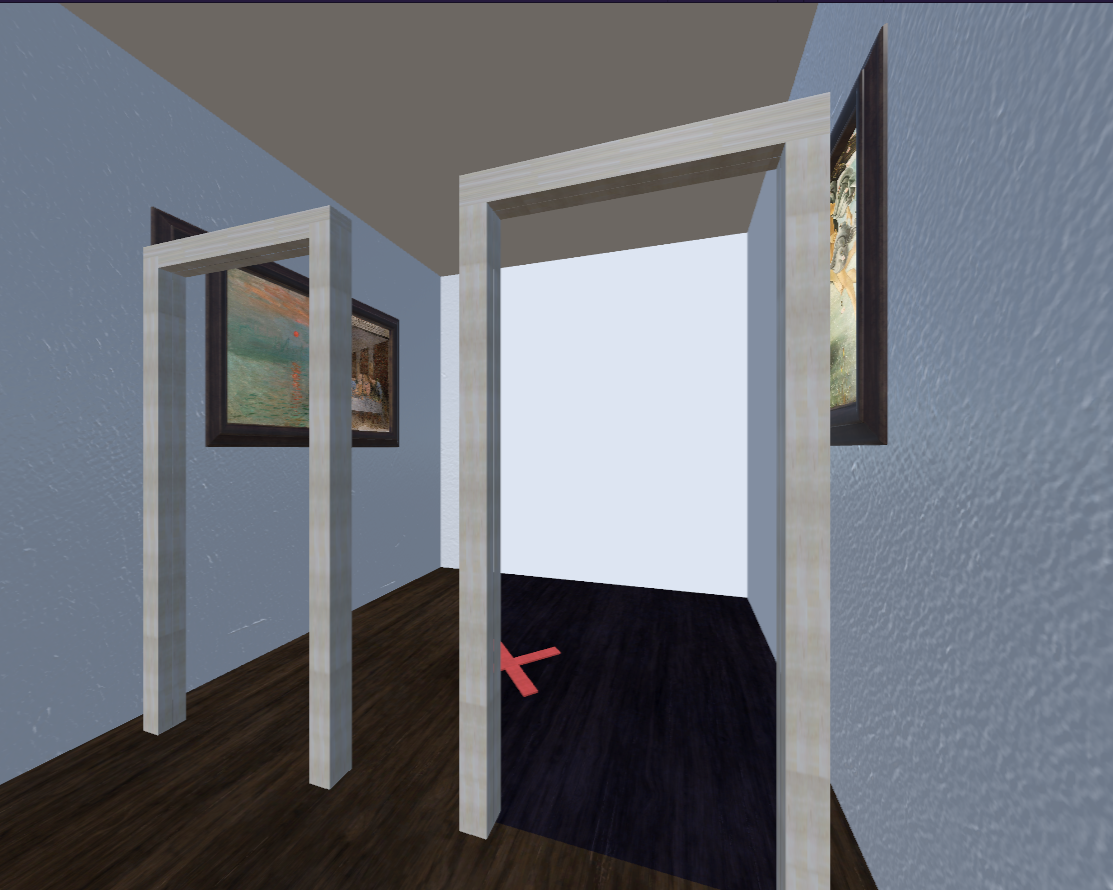
\includegraphics[width=0.6\textwidth]{NOVAthesisFiles/Images/screenshots/traditional-portal.PNG}
     \caption[The Traditional Portal.]
     {The Traditional Portal.}
     \label{fig:trad-portal-sc}
\end{figure}

A main \textit{Portal} script component handles the logic that controls the positioning of the cameras, as well as the detection and 
teleportation of a \textit{PortalTraveller} through the aforementioned trigger colliders, the rendering of the portal preview onto 
the screens and the linking between portals. The script provides a manual input of the portal that is to be linked with the portal that 
holds the script. 
With the portals linked, it is possible to calculate the positioning of the cameras using transform matrices. 
The equation for the positioning of each of the two portal cameras is:

\[
\mathbf{T}_{\text{portalCamera}} =
\mathbf{M}_{\text{thisPortal}} \cdot
\mathbf{M}_{\text{linkedPortal}}^{-1} \cdot
\mathbf{T}_{\text{eyeCamera}}
\]

where: 

\begin{itemize}
    \item $\mathbf{T}_{\text{traveller}}$ = the transform in world space of the camera correspondent with the user's eye
    \item $\mathbf{M}_{\text{linkedPortal}}^{-1}$ = inverse of the linked portal's world transform
    \item $\mathbf{M}_{\text{thisPortal}}$ = current portal's world transform
    \item $\mathbf{T}_{\text{portalCamera}}$ = the transform of the camera used to render the portal view
\end{itemize}

    
Given the interaction design of this portal type, this portal does not change states at any point during the interaction, as users only 
pass through it to go to their pertained destination.
    
\begin{figure}[t]
    \centering
     
\includegraphics[width=0.75\textwidth]{NOVAthesisFiles/Images/placeholder.pdf}
     \caption[Traditional Portal components.]
     {Traditional Portal components.}
     \label{fig:trad-portal-comp}
\end{figure}
    
\subsection{Movable Portals}
\label{sec:mov-portals}

The Movable Portal extends the functionality of the Traditional Portal, with additional features that allow it to be repositioned and 
placed within the environment, as described in Section~\ref{sec:mov-portal-design}. Figure~\ref{fig:mov-portal-sc} demonstrates the implemented interaction of the 
technique and the component structure of this portal technique is shown in Figure~\ref{fig:mov-portal-comp}.

The elements of the Traditional Portal are fully maintained: the frame, the two screens, the two cameras, and the core portal script 
on the parent object. This variant differs by introducing two handles on the portal's frame, which include colliders to enable interaction.
It also defines a valid area where the portal can be placed when grabbed. In addition to the base functionality, a dedicated
\textit{MovablePortal} script manages all behaviors related to the interaction with this portal, ensuring that its movement and placement 
follow the defined constraints.

The \textit{MovablePortal} scrip component, takes the following three states necessary for this portal: \textbf{1.~Start} - when the portal is 
against the wall before being interacted - \textbf{2.~Held} - when it is being held by the user - and \textbf{3.~Placed} - when it has been 
placed in the valid area.
\begin{figure}[t]
    \centering
    \mbox{} \hfill
    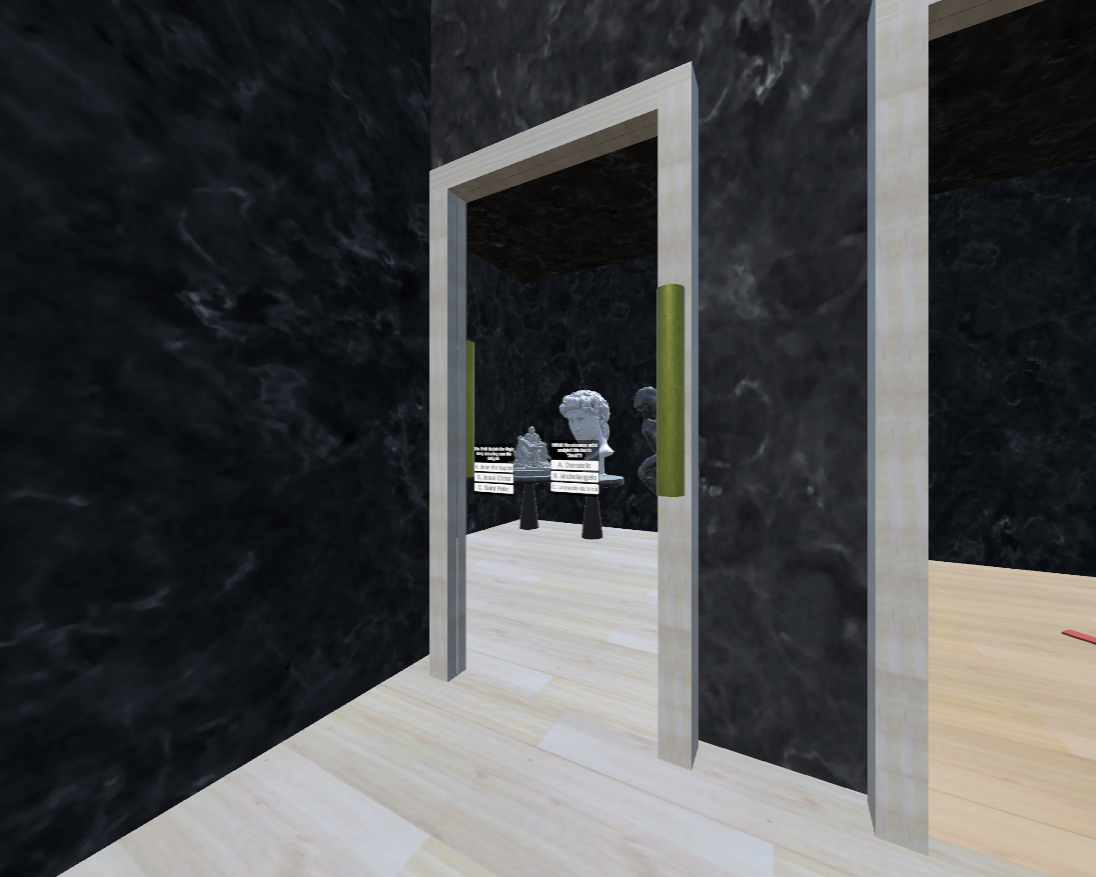
\includegraphics[width=.45\linewidth]{NOVAthesisFiles/Images/screenshots/mov-portal-a.png}
    \hfill
    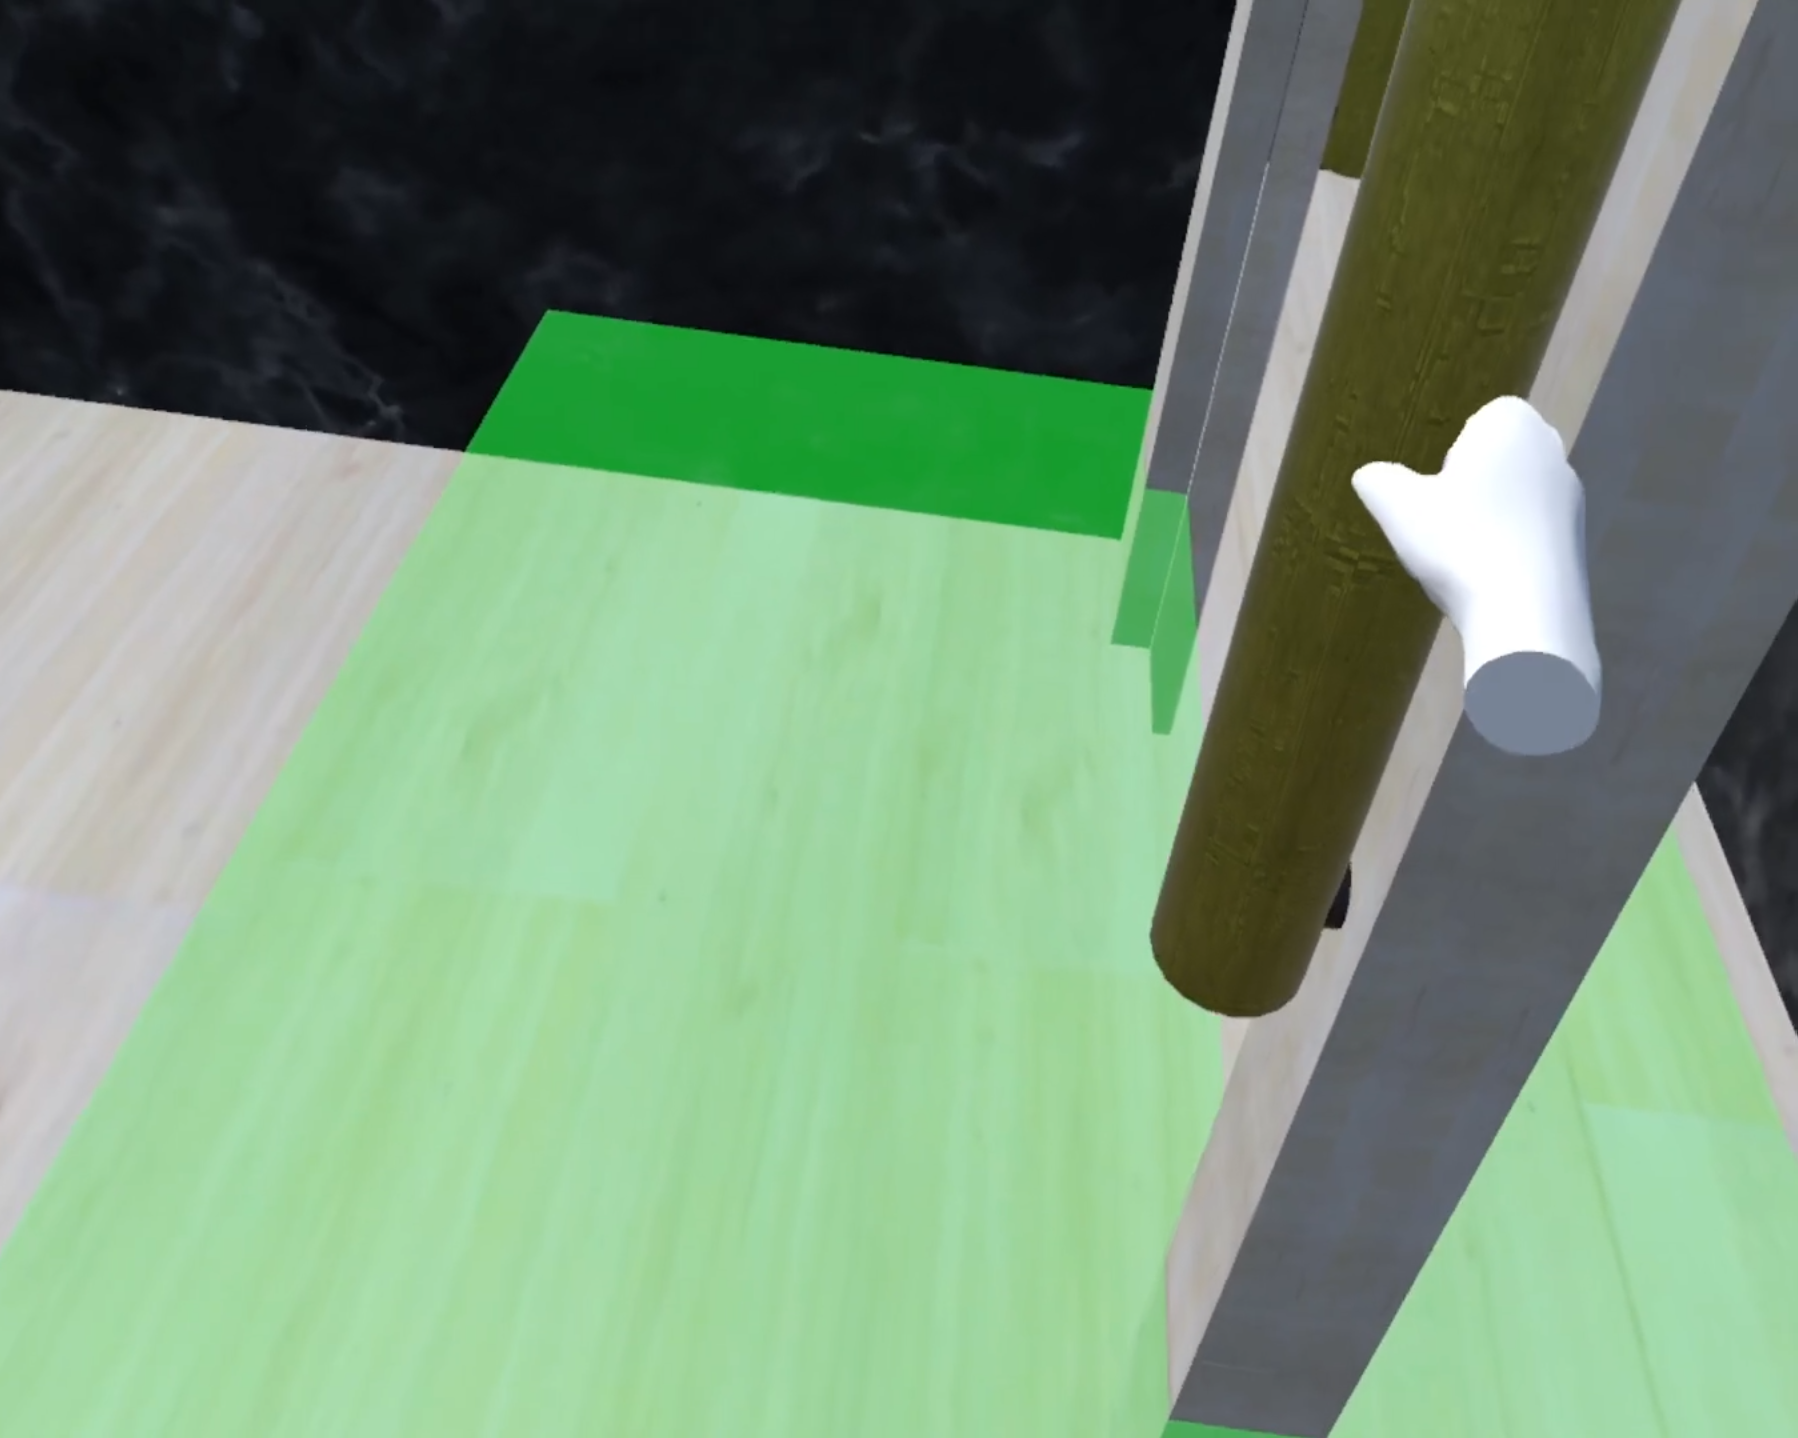
\includegraphics[width=.45\linewidth]{NOVAthesisFiles/Images/screenshots/mov-portal-b.png}
    \hfill \mbox{}
    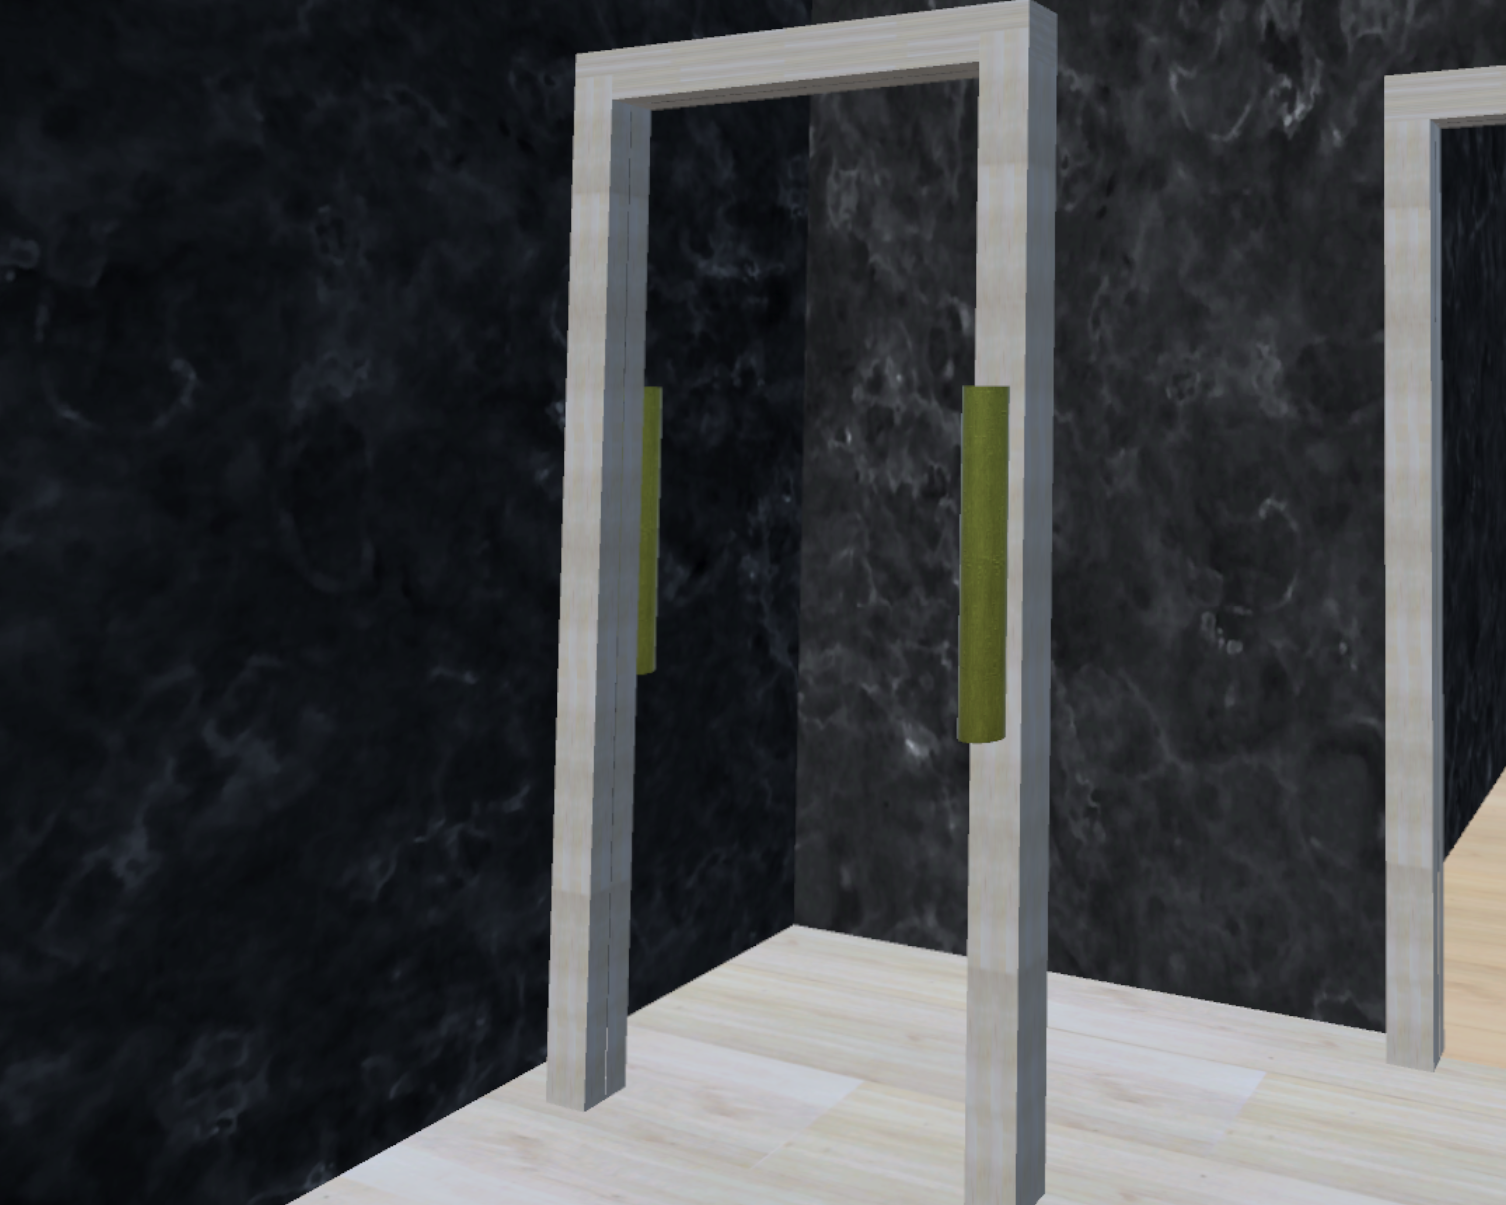
\includegraphics[width=.45\linewidth]{NOVAthesisFiles/Images/screenshots/mov-portal-c.png}
    \caption{The interaction sequence for the Movable Portal: (a) Initially, the portal is placed against the wall with a rotated continuous preview. (b) The user grabs the portal with their virtual hand through the golden-handle. A green valid area is displayed to show the user where they may place the portal. (c) The user places the portal by letting go of the golden-handle. The preview rotates to match the position of the user.}
  \label{fig:mov-portal-sc}
\end{figure}

\begin{figure}[t]
    \centering
     
\includegraphics[width=0.75\textwidth]{NOVAthesisFiles/Images/placeholder.pdf}
     \caption[Movable Portal components.]
     {Movable Portal components.}
     \label{fig:mov-portal-comp}
\end{figure}

When the portal is placed against a wall in the Start state, it renders a preview of the connected space, similar to Traditional Portals. 
However, to create the illusion of a continuous space, the preview is mirrored along the y-axis. This is effectively done by 
spinning the portal 180 degrees on the y-axis, changing the $M_{\text{thisPortal}}$ matrix from the aforementioned equation and, 
by consequence, inverting the positioning of the cameras of the linked portal. The teleport functionalities of the \textit{Portal} script 
are interrupted, preventing users from reaching the edge of their physical tracking space.

The transition to the 'Held' state happens when the user grabs the handle of the Movable Portal. Whenever a user does a grab/pinch gesture 
with their virtual hand while it is positioned within the collider of the handle, an Event is triggered, which in
turn triggers the portal's transition to the 'Held' state. 

In the 'Held' state, the position of the portal tracks the user's movement for as long as the grab gesture is maintained. 
Additionally, the valid area where the portal may be placed is also rendered and stays so for the duration of this state.
To avoid accidental teleportations, the teleport functionalities of the \textit{Portal} script remain paused, 
certifying users don't accidentally clip into the portal while holding it.

To place the portal and transition it to the 'Placed' state, the user must release it within the bounds of the valid area by ending the 
grabbing gesture. To verify if the position of the portal is valid, the following inequalities are used:
\[
P \in \text{zone} \iff 
\begin{cases} 
|\,x_p - c_x\,| \le \frac{w}{2} \\[2mm]
|\,z_p - c_z\,| \le \frac{d}{2}
\end{cases}
\]

where:
\begin{itemize}
    \item $P = (x_p, y_p, z_p)$ is the point transformed into the local space of the zone: $P' = T^{-1} P$.
    \item $C = (c_x, c_y, c_z)$ is the center of the valid zone in local coordinates.
    \item $w, d$ are the width (X-axis) and depth (Z-axis) of the box.
\end{itemize}

If let go in an invalid position, the portal returns to the 'Start' state, returning to its starting position. Otherwise, if let go in a valid 
position, the portal transitions to the 'Placed' state. When 'Placed' the linked portal matches the position of the now placed portal in the $x$ and 
$z$ axis, so that they become overlapped. The rotation of both portals are matched as well, so that the preview reverts to the way it is calculated on Traditional 
Portals, in order to achieve a seamless transition. Once this alignment is complete, the teleport functionality of the \textit{Portal} script resumes.

\subsection{Interactive Door}
\label{sec:interactive-door}

The design of the Interactive Door prioritizes naturalism, being modelled after a familiar real-world object: a door.
Its functionality extends the concept of a standard doorway by enabling dynamic interaction within the environment, 
allowing users to open and close the door at their will, manipulating the space it occupies in the environment 
in an intuitive manner. Figure~\ref{fig:int-door-sc} 
illustrates an example of the implemented interaction, while the component structure supporting this interaction is depicted 
in Figure~\ref{fig:int-door-comp}.

Designed after real-world doors, the Interactive Door is composed of a doorway completed with a panel door featuring a golden handle. 
The two screens on which the preview is rendered are behind the door, nested in the hierarchy of the door object, so that the screens position follow 
the motion the door does when opening or closing. The portal additionally includes the two cameras necessary to render the preview of the linked portal.
To handle the logic of this portal variant, the inclusion of an \textit{InteractiveDoor} script was added to the parent object.

The Interactive Door may be in one of three states: \textbf{1. Closed} - the state before interaction begins, in which the door's transparency 
is dynamic; \textbf{2. Open} - the state after the user initiates the transition by opening the door; and \textbf{3. Following} - the state in 
which the portal is when the door of its linked portal is opened.




\subsection{Revolving Door}
\label{sec:rev-door}

\section{Summary}
\label{sec:summary}
\todo{Completar de acordo como ficar no final}
